\chapter{Draft - não pronto}

\section{RQ1. Com que frequência \textit{breaking changes} surgem nos pacote clientes?}
\label{sec:rq1}

\subsection{Motivation}
\label{mot:rq1}

O \Gls{NPM} contém mais de 11 bilhões de downloads semanais e ultrapassa os 45 bilhões por mês. Esses são usados por milhões de pessoas e projetos por todo o mundo. Entretanto, uma simples \textit{release} que contenha um erro pode afetar uma quantidade imensa de pacotes. Isso se deve ao fato dos pacotes dependerem uns dos outros, direta ou indiretamente.

Para evitar estes erros, o \Gls{NPM} utiliza \textit{strings} de versionamento, baseadas no \Gls{SEMVER} para especificar as versões dos provedores. Isso permite que um provedor publique uma \textit{release} que contenha \textit{breaking changes} sem afetar os clientes das versões prévias. Entretanto, a distinção entre \textit{breaking} e \textit{non-breaking changes} não é totalmente clara \cite{noregrets2018}. Assim sendo, é interessante entender com que frequência os provedores publicam \textit{releases} com \textit{breaking changes}.

Para responder essa questão de pesquisa, serão analisados três pontos: 1) quantas vezes cada provedor publica uma \textit{release} que contém \textit{breaking changes}; 2) em qual nível da \textit{string} de versionamento as \textit{breaking changes} são tipicamente introduzidas, de acordo com o \Gls{SEMVER}; 3) qual o percentual de clientes que atualizam para uma versão com \textit{breaking changes}.

Para analisar todos esses pontos, os pacotes sorteados serão clonados do \textit{GitHub}, atualizado o \textit{index} e os arquivos na \textit{Working Tree} para o \textit{timestamp} da \textit{release}, atualizado a versão de cada um dos provedores no \textit{package.json} e executado os comandos \textit{npm install} e \textit{npm test}. Então, o resultado da execução será salvo juntamente com as  versões do \textit{Node.JS}.

\subsection{Approach}
\label{apr:rq1}

Um \textit{stack trace} contém as informações sobre as subrotinas de um programa. Quando os comandos \textit{npm install} e \textit{npm test} resultam em erro, o \Gls{NPM} todas as chamadas de função, incluindo as invocações para os provedores. A Figura \ref{fig:trace} mostra um exemplo genérico de um \textit{stack trace} exibido pelo \Gls{NPM} após a ocorrência de um erro.

\begin{figure}
    \centering
    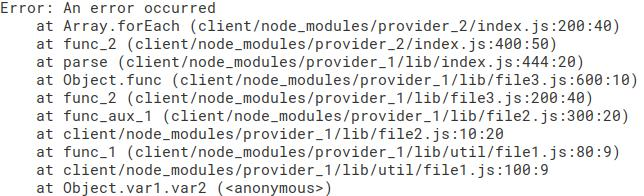
\includegraphics[scale=0.7]{figuras/stack_trace.jpeg}
    \caption{Generic stack-trace}
    \label{fig:trace}
\end{figure}{}

O \textit{stack trace} é a base da analise de um erro. A primeira etapa da análise de um erro é diferenciar entre um erro que foi causado pelo próprio pacote cliente, no qual não houve influência de nenhum provedor, e um erro que foi causado por algum dos provedores. Esta análise foi realizada de duas maneiras diferentes.

A primeira maneira foi verificar diretamente no \textit{stack trace} do erro e procurar as chamadas de função para os provedores. Quando não há chamada para os provedores no \textit{stack trace}, provavelmente o erro não se trata de uma \textit{breaking change}. Então, a falha pode estar apenas no código do cliente. Para confirmar isto, foi procurado no \textit{GitHub} do cliente pelos próximos \textit{commits} após a data da \textit{release} e verificado se o desenvolvedor realizou alguns \textit{commits} com a intenção de consertar algum erro. Se sim, o código do cliente foi alterado para verificar se as modificações presentes nos \textit{commits} realmente refletem a correção do erro. Entretanto, alguns tipos de erros já indicam exatamente onde o erro aconteceu. São os \textit{SyntaxError} e \textit{ReferenceError}, no qual já se sabe onde e porque ocorreu. O Código \ref{cod:syntax:error} mostra um exemplo deste tipo de erro.

\begin{lstlisting}[style=Javascript, label=cod:syntax:error, caption={Código com um Reference Error}]
const a = 0 = 0;
\end{lstlisting}

A segunda maneira é quando o erro indicava a presença de \textit{breaking changes}. Isto se evidenciava quando havia chamadas para os provedores no \textit{stack trace}. Entretanto, as chamadas para \textit{frameworks} de teste, como o \textit{Mocha, Instanbul, Jasmine} entre outros, ou automatizadores de tarefas, o \textit{Grunt} por exemplo, não evidenciam diretamente a presença de \textit{breaking changes} uma vez que eles apenas iniciam a execução do pacote e deveriam estar ali. Porém, não foram totalmente descartados de apresentar \textit{breaking changes}. Assim, quando havia algum provedor no \textit{stack trace}, provavelmente se tratava de um caso de \textit{breaking change}.

O melhor local para se confirmar esta evidência é o \textit{GitHub}. Neste, os repositórios dos pacotes contêm todo o histórico de desenvolvimento. E muitas maneiras foram utilizadas para recuperar as informações necessárias. A primeira e mais fácil foi procurar nos arquivos registros de alterações, os comumente nomeados de \textit{CHANGELOG.md} ou \textit{HISTORY.md}. A proposta destes arquivos é manter uma lista ordenada cronologicamente das alterações significativas ao longo do desenvolvimento do projeto. E uma das informações muito importantes que são descritas nesses registos são as \textit{breaking changes}. Por exemplo, a versão \textit{5.0.0} do projeto \textit{Mocha} contém uma \textit{breaking change} que foi documentada no \textit{CHANGELOG.md}\footnote{https://github.com/mochajs/mocha/blob/master/CHANGELOG.md\#500--2018-01-17} de acordo com a Figura \ref{fig:bc_documentation} (a). Outro tipo de documentação equivalente aos \textit{changelogs} são as \textit{releases-notes} que seguem o mesmo propósito, como pode ser visualizado na Figura \ref{fig:bc_documentation} (b) como o projeto \textit{npm-wpxml2md} documentou \textit{breaking changes} nas \textit{releases-notes}.

\begin{figure}
    \centering
    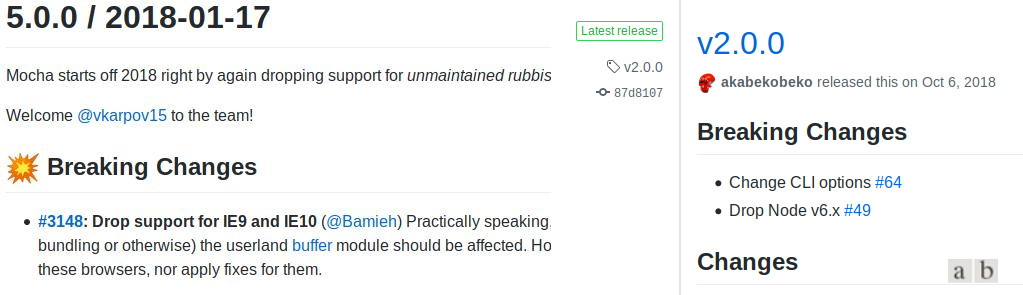
\includegraphics[scale=0.45]{figuras/bc_documentation.jpeg}
    \caption{Breaking Change documentation in CHANGELOG and release-notes}
    \label{fig:bc_documentation}
\end{figure}{}

Assim, foi observado a versão do provedor que possivelmente causou o erro e foi verificado no seu \textit{CHANGELOG}/\textit{releases-notes} -- caso existisse -- se contém alguma informação pertinente ao erro que foi apresentado pelo \gls{NPM} quando os comandos \textit{npm install} e \textit{npm test} resultou em erro. Então foi salva as informações sobre este erro: a versão que iniciou, a versão que foi corrigido, uma breve descrição para facilitar a classificação da \textit{breaking change}, quem consertou o erro: cliente ou provedor; o tempo total até ser corrigido, quantas \textit{releases} o provedor levou para corrigir e em qual nível do \gls{SEMVER} o erro foi consertado.

Entretanto, apenas 46\% dos repositórios contêm algum dos dois registros. Assim, uma alternativa foi verificar nas \textit{issues} dos repositórios. Nestas, muitas informações foram encontradas. E muito mais, pois há uma grande rede interligada de \textit{issues} e \textit{pull-requests} no qual uma \textit{issue} é marcada em outra \textit{issue}, que é marcada em um \textit{pull-request} e assim por diante. Deste modo, uma simples \textit{issue}/\textit{pull-request} contém muita informação.

Um ponto que foi muito importante para descobrir as versões que foram introduzidas as \textit{breaking changes} é a instalação de versões prévias e sucessivas dos provedores. Com isso, foi possível testar a partir de qual versão o erro foi introduzido e consertado e descobrir qual foi o verdadeiro provedor causador do erro. Também, alguns outros recursos foram utilizados para buscar as informações desta questão de pesquisa, tais como, o uso da ferramenta \textit{npm-diff}\footnote{https://github.com/danielventurini/npm-diff}, que provê os \textit{diff} do código entre duas \textit{releases} de um determinado projeto, no qual foi verificado o que realmente foi introduzido e o que foi removido com mais detalhes.

A Figura \ref{fig:step_analyze} exemplifica as técnicas utilizadas para responder esta questão de pesquisa.

\begin{figure}
    \centering
    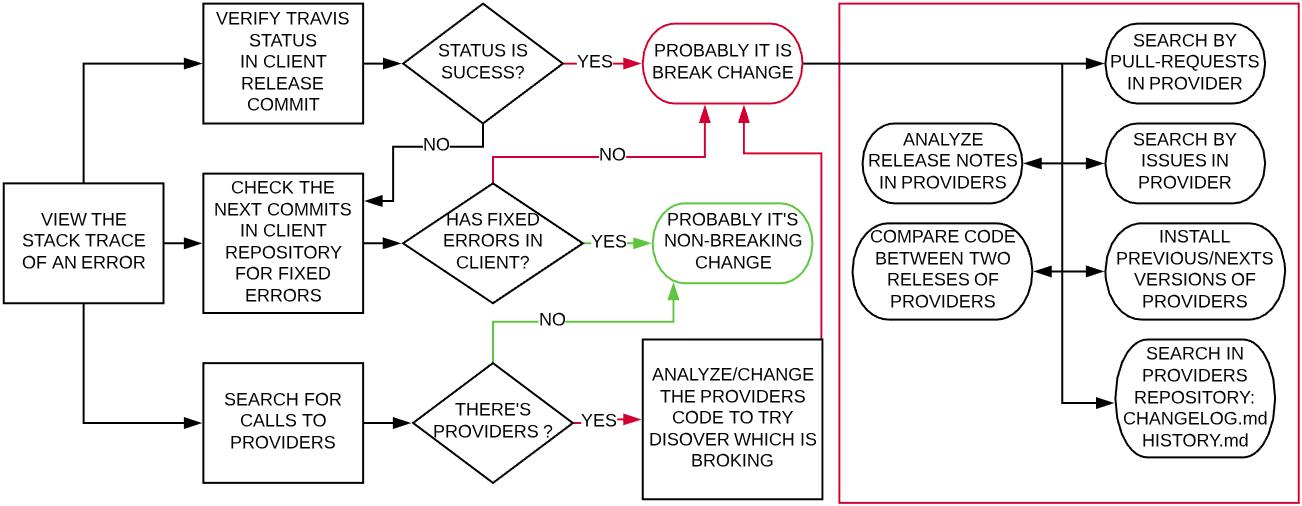
\includegraphics[scale=0.35]{figuras/step_analyze.jpeg}
    \caption{Steps to analyze an error}
    \label{fig:step_analyze}
\end{figure}

Vale ressaltar que alguns sistemas integrados ao \textit{GitHub} auxiliaram na investigação. Esses sistemas são o \textit{Travis, Jenkins, Codeship, CicleCI} etc. que, quando o desenvolvedor realizou o \textit{commit}, esses sistemas executaram o \textit{npm install} e o \textit{npm test}. Eles colaboraram da seguinte maneira: se o \textit{commit} da \textit{release} teve sucesso na execução \textit{npm install} e \textit{npm test} e, ao executá-los nesta pesquisa resultou em erro, indica que há uma \textit{breaking change}, uma vez que o código do cliente está no mesmo \textit{index} da \textit{working tree} da \textit{release}, apenas os provedores que foram atualizados e, para o range aceito, geraram erros, resultando em \textit{breaking changes}. Entretanto, nem todos os projetos utilizavam estes sistemas integrados, mas quando dispunham, foi de grande valia.

Outro detalhe importante se refere aos projetos que utilizavam algum tipo de sistemas terceiros como o \textit{MySql, CouchDB, Redis} etc. Então, quando foi gerado um erro pela falta de um destes, fez-se a habilitação destes e o pacote foi re-executado. Entretanto, quando os pacotes requeriam previamente uma configuração para executar, tais como a criação de tabelas em banco de dados, esta configuração foi feita, seguindo o modelo disponibilizado pelo desenvolvedor afim de realizar os teste, e novamente foi executado o pacote.

Então, para todas as \textit{releases} analisadas manualmente, foi salvo as seguintes informações:

\begin{enumerate}
    \item Em que local o erro foi documentado: \textit{issue, changelog, pull-request} etc;
    \item Quem consertou o erro: cliente ou providor;
    \item Em qual nível do \textit{SEMVER} o erro foi reparado;
    \item Quanto tempo o erro levou até ser corrigido; e
    \item Por quantas \textit{releases} o erro persistiu.
\end{enumerate}{}

Porém, nem todas as informações puderam ser recuperados, uma vez que nem todos os projetos contêm todos estes dados. Por exemplo, quando um caso de erro nunca foi consertado, nem pelo provedor nem pelo cliente, as informações 2, 3, 4 e 5 não existem. Também, alguns pode haver casos em que a documentação do erro não foi encontrado em lugar algum.

\subsection{Findings}
\label{fin:rq1}

\subsubsection{De todos os projetos, 11\% foram impactados por \textit{breaking change}}

\subsubsection{De todos os projetos afetados, 13\% apresentaram mais de uma \textit{breaking change}}

%---------------------------------------------------%
\section{RQ2. Quais são os problemas no pacote provedor que causam \textit{breaking change}?}
\label{sec:rq2}

\subsection{Motivation}
\label{mot:rq2}

Produzir códigos de teste é uma das estratégias mais importantes para garantir que um projeto esteja executando da maneira esperada. Entretanto, uma pesquisa realizada por \citeonline{uncovered} mostrou que os projetos \textit{Javascript} não possui \textit{scripts} de testes em 22\% da base estudada; 40\% dos projetos puramente clientes; e 3\% dos projetos servidores. Além disso, nem sempre os testes possuem cobertura total do projeto. Por esse fato, ha grande probabilidade de um erro ser descoberto apenas em tempo de execução pelos clientes.

Em linguagens fortemente tipadas, tais como \textit{Java} e \textit{C Sharp}, uma simples alteração errônea na estrutura pode ser facilmente identificada em tempo de compilação e pelo próprio desenvolvedor. Por exemplo, uma alteração na estrutura de uma classe em \textit{Java} já gera um erro de compilação dependendo de como essa é utilizada pelos clientes. Por isso, os provedores podem conter variados tipos de erros. Uma simples linha escrita semanticamente errada, por exemplo, pode causar no encerramento apenas em tempo de execução, uma vez que os códigos \textit{Javascript} não são compilados. Também, erros de conexão, arquivos inexistentes, provedores removidos, funções renomeadas etc. são outros tipos de defeitos que o provedor pode apresentar. Pelo fato dos pacotes dependerem uns dos outros, os tipos de erros se repetem com frequência em vários casos. Por isso, é interessante categorizar e quantificar os erros para descobrir quais são os casos mais frequentes nos casos de \textit{breaking changes}.

Para responder essa questão de pesquisa, será analisado caso a caso dos erros e as \textit{breaking changes} serão categorizadas pelo tipo da \textit{breaking change}. Também, os tipos serão quantificados pela categoria, pelo número de \textit{releases} afetadas e pelo número de clientes que sofreram com uma determinada categoria de \textit{breaking change}.

\subsection{Approach}
\label{apr:rq2}

Cada um dos casos de erro para os comandos \textit{npm install} e \textit{npm test} foram analisados manualmente. O objetivo era descobrir o real motivo que origino o erro e agrupa-los por suas similaridades. Isso, porque o \textit{stack trace} sempre apresenta o erro de uma maneira genérica. Então, as vezes, a mensagem de erro pode induzir a interpretação errônea do real motivo que originou a falha. Por exemplo, a Figura \ref{fig:error_category} mostra dois casos no qual uma função foi renomeada pelo provedor. Entretanto, previamente não está claro o real motivo dos erros, apesar da mensagem do \textit{stack trace}.

\begin{figure}[!h]
    \centering
    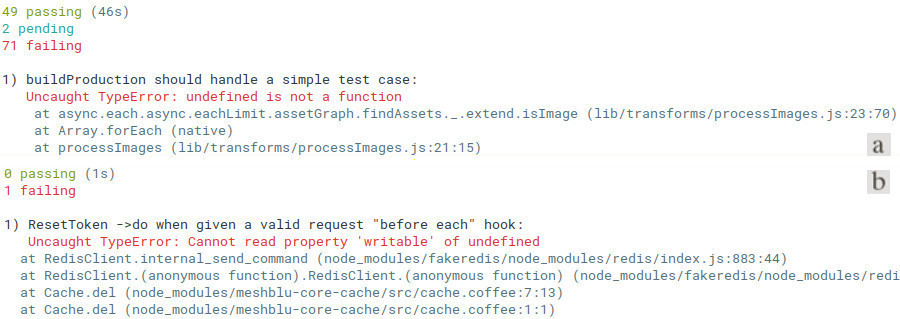
\includegraphics[scale=0.5]{figuras/error_category.jpeg}
    \caption{Two error caused by a renamed function}
    \label{fig:error_category}
\end{figure}

A mensagem do primeiro erro (a) deixa claro que se trata de uma invocação a uma função inexistente, ou seja, o cliente tentou acessar uma variável como uma função quando essa não era. Mas somente pela mensagem do \textit{stack trace} é possível deduzir que uma função foi renomeada no provedor. Já no segundo erro (b), o \textit{stack trace} não indica que se trata de uma função renomeada. Somente após uma análise deste caso é que foi possível concluir que o erro aconteceu por uma invocação a uma função que não existia, haja visto que fora renomeada. Assim, apesar de mensagens de erro diferentes, foram classificados pelo seu real motivo para que fosse possível quantificar os principais problemas no código do provedor.

Por isso se fez necessário a análise manual para reconhecer os reais motivos de cada caso de erro.

\subsection{Findings}
\label{fin:rq2}

%---------------------------------------------------%
\section{RQ3. Como os pacotes clientes se recuperam das breaking change?}
\label{sec:rq3}

\subsection{Motivation}
\label{mot:rq3}

Uma vez que uma \textit{breaking change} é introduzida o provedor deve se recuperar desta. Isso se faz necessário pois, no ecossistema \gls{NPM}, no qual centenas de milhares de pacotes estão conectados, uma simples \textit{release} com erro pode ocasionar na quebra de muitos clientes. Isso ocorreu com um pacote chamado \textit{left-pad}\footnote{https://blog.npmjs.org/post/141577284765/kik-left-pad-and-npm}. Esse foi removido do \textit{NPM} por seu desenvolvedor e impactou milhares de projetos em apenas 2.5 horas incluindo \textit{babel}\footnote{https://github.com/babel/babel} e \textit{atom}\footnote{https://github.com/atom/atom}.

A responsabilidade para corrigir uma errônea \textit{release} é do provedor. Entretanto, as vezes, o provedor deixa dar a manutenção por algum motivo. Então, os clientes recebem esta responsabilidade, uma vez que o erro no seu provedor pode afetar os seus clientes. No caso do \textit{left-pad} o provedor nunca publicou uma nova \textit{release} e, para que todos os pacotes continuassem a executar normalmente, um dos clientes publicou um pacote com o mesmo nome e mesmo código, uma vez que a política para nomes de pacotes permitia este feito e o pacote original continha uma licença de código aberto.

No entanto, como os provedores evoluem independentemente dos clientes, erros e vulnerabilidades são difíceis de rastrear e corrigir nos clientes. Mesmo quando as vulnerabilidades podem ser corrigidas com a atualização para uma versão mais recente do provedor, pode haver incompatibilidades de \textit{API} -- entre outras incompatibilidades -- com os clientes que deve ser resolvido manualmente \cite{Foo:2018:ESC:3236024.3275535}. Assim, o cliente dificilmente irá conseguir ter sucesso quanto a resolução do erro no provedor. Então, uma alternativa para o cliente é mudar de provedor buscando por um que atenda as necessidades que não fora atendidas pelo provedor prévio.

Para responder a questão de pesquisa final, foi analisado três pontos: 1) o que aconteceu para que o provedor não pudesse consertar o erro; 2) como o cliente consertou o erro: no seu código ou notificando o provedor através de \textit{issues} e \textit{pull-requests}; 3) quantas vezes o cliente teve que realizar a correção dado que o provedor não a fez. Todas as informações sobre esta questão de pesquisa estão nos \textit{commits}, \textit{issues}, \textit{pull-requests}, \textit{changelogs} e \textit{releases-notes} dos repositórios do cliente e do provedor.

\subsection{Approach}
\label{apr:rq3}

Uma vez que os clientes se recuperaram de um erro, há duas maneiras para se obter informações sobre esta recuperação. A primeira maneira é quando o provedor corrige seu código e o cliente apenas atualiza sua \textit{string} de versionamento no \textit{package.json}, se precisar. Para o provedor consertar o erro, deve haver uma \textit{issue} no seu repositório. A segunda maneira é quando o próprio cliente conserta o código. Neste caso, o cliente pode corrigir o código do provedor e realizar um \textit{pull-request}. Também, o cliente pode alterar apenas o seu código para que execute normalmente com a \textit{release} errônea do cliente. Há casos também no qual nem o cliente nem o provedor faz nada para consertar o erro.

Todas as informações sobre esta questão de pesquisa foi recuperada do \textit{GitHub}. As informações foram encontradas em \textit{CHANGELOGs, release-notes, issues} e \textit{pull-requests}. Se os \textit{CHANGELOGs} contêm informações sobre os erros consertados, geralmente, as \textit{issues} são marcadas, como mostra a Figura \ref{fig:bc_documentation}. A partir das \textit{issues} uma grande quantidade de informações podem ser recuperadas. Pois, assim como o código de um projeto fica emaranhado com o código no restante do ecossistema ao qual ele pertence, o mesmo acontece com as \textit{issues}. Uma manifestação disso é que muitas \textit{issues} abertas em um projeto são vinculadas a \textit{issues} relacionadas, em projetos iguais ou diferentes, pois os desenvolvedores estão rastreando as causas de um problema \cite{Zhang:2018:WIL:3242887.3242891}. Da mesma maneira, os \textit{pull-requests} que são relacionados ao mesmo problema são marcados, abrangendo ainda mais a quantidade de informações que podem ser recuperadas. Todas estas informações corroboram para descobrir como a \textit{breaking change} foi tratada/consertada e quem -- cliente ou provedor -- a consertou, caso tenha sido consertada.

Os \textit{commits} são alternativas para as \textit{issues} quando a busca se dá no repositório do cliente. Os \textit{commits} contém todas as alterações de cada arquivo, incluindo o arquivo principal \textit{package.json}, no qual se pode ver todos as atualizações dos provedores. Sobre os \textit{commits}, mensagens do tipo \textit{update dependencies, fix dependencies, fix errors} etc. sugerem que algum provedor foi atualizado para consertar algum erro ou um erro foi consertado diretamente no código do cliente. Esta informações é muito importante, uma vez que o provedor corrigiu a \textit{breaking change} e o cliente apenas o atualizou. Assim, as mensagens dos \textit{commits} auxiliaram para descobrir os reais motivos da atualização -- ou retrocesso da versão.

\subsection{Findings}
\label{d_fin:rq3}